\section{Visning af kort}
\label{sec:visningAfKort}

Når brugeren navigerer kortet og bliver på samme zoom-niveau vil der være dele af kortet som allerede er tegnet, der skal tegnes igen. Der er et overlap mellem det gamle og det nye udsnit af kortet (figur~\ref{figur:visningAfKort1}).

\begin{figure}[h]
	\centering
	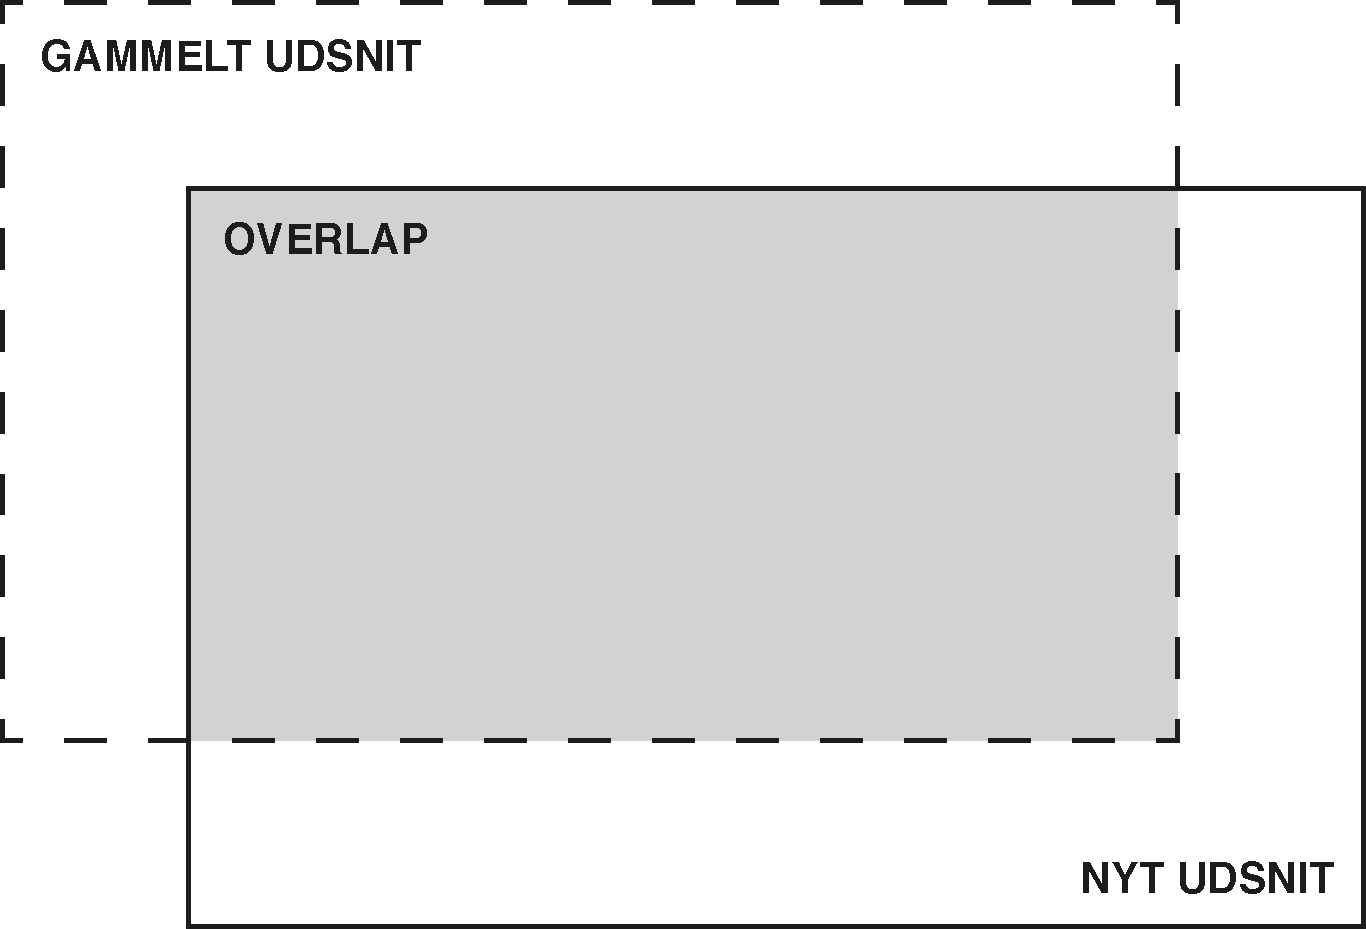
\includegraphics[width=0.5\textwidth]{visningAfKort1}
	\captionsetup{width=0.8\textwidth}
	\caption{Overlap mellem gammelt og nyt udsnit.}
	\label{figur:visningAfKort1}
\end{figure}

Til at starte med tegnede vi hele udsnittet, inklusiv overlap, men det viste sig ikke at være hurtigt nok, og responstiden blev problematisk. Det blev derfor besluttet at vi havde brug for en mere effektiv løsning, der kun tegner den del af et nyt udsnit der ikke overlapper med det gamle udsnit.

Dette afsnit er skrevet på et tidspunkt hvor vores implementering af quadtræer ikke var optimal. En af ulemperne ved denne implementation var, at den returnerede en margin af vejstykker uden om den rektangel der var efterspurgt. Denne margin udggjorde i mange tilfælde helt op til 70-80\% af de returnerede vejstykker. Efter optimeringen er denne ulempe ikke eksisterende.

Analyserne i dette afsnit tager udgangspunkt i implementeringen før optimeringen, og der er derfor lagt stor vægt på at ovennævnte ulempe eksisterede. Analyserne er dog fortsat relevante, men gevinsten ved at bruge de nævnte løsninger er langt mindre end den var før optimeringen.

\subsection{Cache og forskydning}
\label{subsec:cacheOgForskydning}

Den første løsning der blev overvejet var at gemme et billede af det gamle udsnit til en cache og forskyde det således at det lå rigtigt i forhold til det nye udsnit (figur~\ref{figur:visningAfKort2}). Efterfølgende tegnes den del af udsnittet som ikke er inkluderet i overlappet.

\begin{figure}[h]
	\centering
	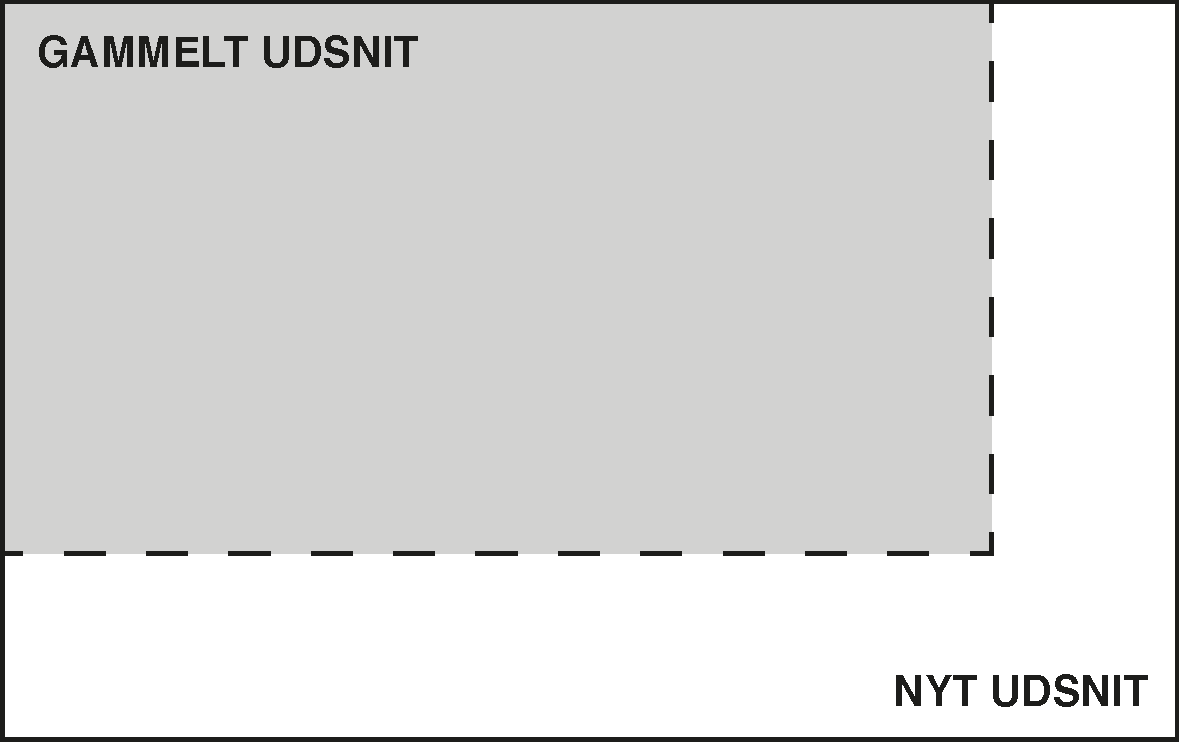
\includegraphics[width=0.5\textwidth]{visningAfKort2}
	\captionsetup{width=0.8\textwidth}
	\caption{Det gamle udsnit ligger forskudt inde i det nye udsnit.}
	\label{figur:visningAfKort2}
\end{figure}

Denne løsning var meget simpel, og vi formoder den havde været nem at implementere. Den havde dog en række klare ulemper, hvilket førte til at vi ikke implementerede den:

\begin{itemize}
	\item Hvis brugeren navigerer tilbage til et udsnit de allerede har set skal dette udsnit tegnes igen.
	\item Der skal gemmes billeddata til en cache hver gang udsnittet ændrer sig, således at denne data kan gentegnes som en del af det næste udsnit.
	\item De udsnit der skal tegnes er tynde, hvilket skaber stor ineffektivitet som følge af den måde som vejstykker hentes fra quadtræer (figur~\ref{figur:visningAfKort3}).
\end{itemize}

\begin{figure}[h]
	\centering
	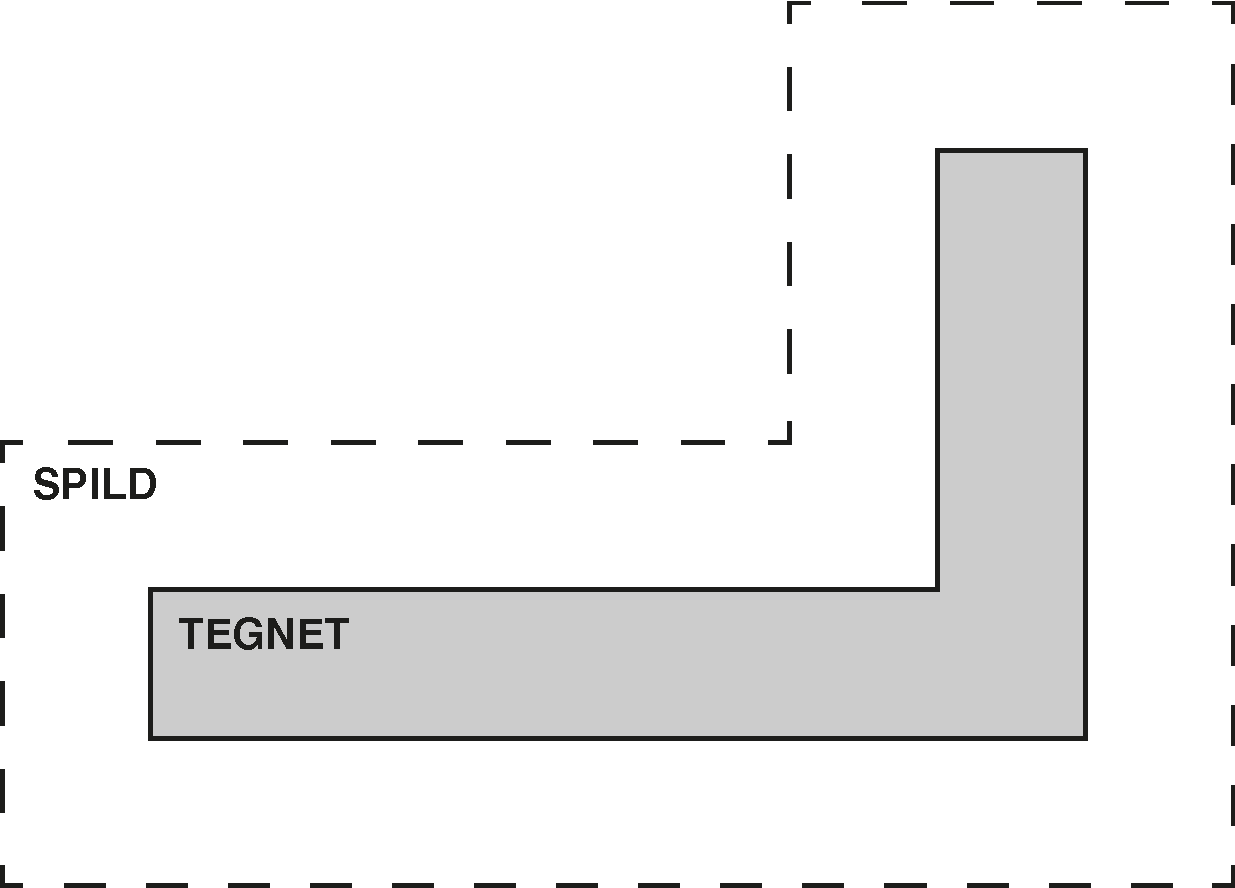
\includegraphics[width=0.5\textwidth]{visningAfKort3}
	\captionsetup{width=0.8\textwidth}
	\caption{Stort spild ved hentning af vejstykker fra quadtræer.}
	\label{figur:visningAfKort3}
\end{figure}

\subsection{Anden løsning}
\label{subsec:andenLoesning}

Den anden løsning vi overvejede, og den vi endte med at implementere, var inspireret af online kort-programmer som for eksempel Google Maps og OSM. Det centrale koncept i denne løsning er at dele kortet op i en masse små rektangler bestående af bitmap data (tiles). Når der er zoomet langt ud udgøres kortet af få tiles, og når der er zoomet langt ind udgøres kortet af mange tiles (figur~\ref{figur:visningAfKort4}). Når der skal tegnes et udsnit tegnes de tiles der er indenfor udsnittet.

\begin{figure}[h]
	\centering
	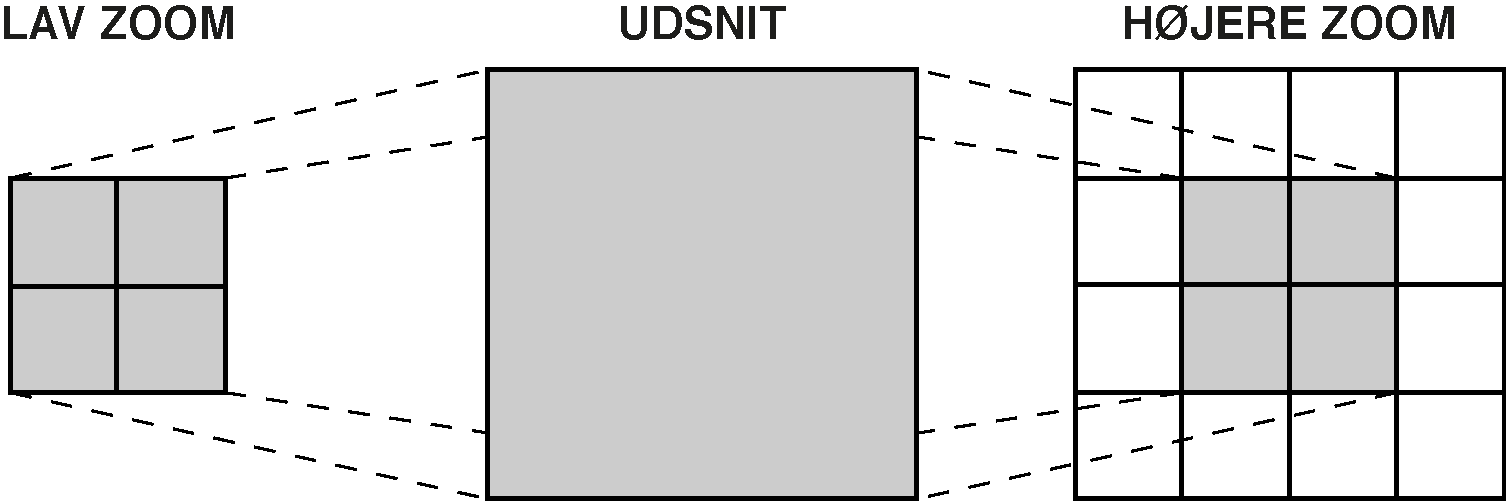
\includegraphics[width=0.9\textwidth]{visningAfKort4}
	\captionsetup{width=0.8\textwidth}
	\caption{Antallet at tiles som kortet udgøres af er afhængigt af zoom.}
	\label{figur:visningAfKort4}
\end{figure}

Denne løsning løser helt eller delvist problemerne ved den ovenstående løsning:

\begin{itemize}
	\item Da de tegnede data er strukturerede, og det er dermed muligt at gemme dem og vise dem igen når det er relevant.
	\item Der skal kun gemmes billeddata til et lager af tiles når der bliver tegnet nye tiles.
	\item De udsnit der skal tegnes er firkantede og har en vis størrelse, hvilket gør problemet med overflødig data mindre.
\end{itemize}

\subsection{De tre planer}
\label{subsec:deTrePlaner}

Når løsningen med tiles anvendes er der tre rektangulære planer der skal tages højde for:

\begin{itemize}
	\item \textbf{Model}: Er 1000 enheder langt på den længste led. Ændrer aldrig størrelse.
	\item \textbf{Tiles}: Er dimensioneret efter et bitmap der ville kunne indeholde tiles for hele det aktuelle zoom-niveau. I praksis bliver sådant et bitmap aldrig oprettet, blot tiles som repræsenterer fragmenter af dette bitmap. Ændrer størrelse afhængigt af zoom-niveau.
	\item \textbf{Skærm}: Har samme dimensioner som det vindue som kortet vises i på skærmen. Ændrer størrelse når brugeren ændrer størrelsen på vinduet.
\end{itemize}

\subsection{Udsnit}
\label{subsec:udsnit}

For at holde styr på hvilket udsnit af kortet brugeren kigger på opdateres to uafhængige variable løbende:

\begin{itemize}
	\item \textbf{Center}: En relativ vektor der definerer centrum for udsnittet. Værdierne for center løber fra 0 til 1 på både x- og y-aksen --- altså er $(0.5, 0.5)$ midten af kortet.
	\item \textbf{Zoom}: En relativ værdi der definerer hvor stor en andel af kortet der vises indenfor udsnittets længste side.
	\begin{itemize}
		\item Når zoom er mellem 0 og 1 er der zoomet ind, og udsnittet rummer kun en andel af kortet.
		\item Når zoom er 1 vises hele kortet.
		\item Når zoom er større end 1 er der zoomet ud, og kortet dækker kun en andel af skærmen.
	\end{itemize}
\end{itemize}

Ved hjælp af disse to variable kan det beregnes hvilket udsnit af kortet der er aktuelt. Vi valgte denne løsning som et alternativ til absolutte koordinater for en boks for at opnå øget fleksibilitet, og fordi denne løsning virkede mere intuitiv for os.

\subsubsection{Hvilke tile skal vises}
\label{subsec:hvilkeTilesSkalVises}

Når kortet skal tegnes skal det afgøres hvilke tiles der skal vises på skærmen.

Først beregnes det hvor udsnittet befinder sig på tiles. Dette gøres ved at tage en boks der har samme dimensioner som skærm, og forskyde den i forhold til tiles således at den nu er centeret omkring center. Denne boks kalder vi for sektion (figur~\ref{figur:visningAfKort10}, venstre).

Dernæst beregnes hvilke tiles som sektion overlapper (figur~\ref{figur:visningAfKort10}, højre). Det er disse tiles som skal vises på skærmen.

\begin{figure}[h]
	\centering
	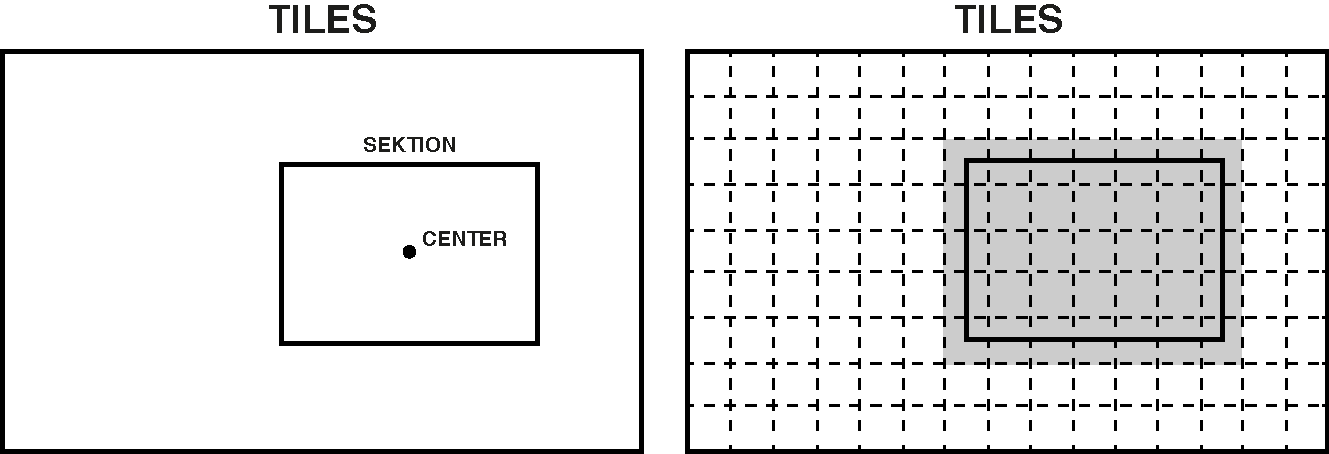
\includegraphics[width=0.9\textwidth]{visningAfKort10}
	\captionsetup{width=0.8\textwidth}
	\caption{De tiles der overlapper med sektion skal vises.}
	\label{figur:visningAfKort10}
\end{figure}

\subsection{Centraliseret lagring af tiles}
\label{subsec:centraliseretLagringAfTiles}

De løsninger vi er inspireret gør to ting markant anderledes end vi gør:

\begin{itemize}
	\item De begrænser antallet af zoom niveauer. Hvis man ikke gør dette er der uendeligt mange zoom-niveauer, og dermed uendeligt mange tiles der potentielt skal lagres.
	\item De har en vedligeholdt database over tiles. Ved at gøre dette undgår de at tegne nye tiles når et udsnit efterspørges --- I stedet hentes tiles fra den centrale database.
\end{itemize}

Vi overvejede en kort overgang at implementere en database løsning, men besluttede os for at det ville være for stor en opgave. Dette ville være en oplagt mulighed for senere optimering af programmet, og kunne både implementeres med en lokal eller en ekstern database.

Eftersom vi ikke anvender en databaseløsning giver det ikke mening at reducere antallet af zoom-niveauer. Da tiles alligevel skal tegnes løbende, ville dette kun være en fordel hvis brugeren vendte tilbage til et udsnit på et zoom-niveau som vedkommende allerede havde set. Da vi ikke tænker at dette scenarie opstår særlig tit, fravalgte vi at begrænse antallet af zoom-niveauer og dermed forringe programmets funktionalitet unødvendigt.

\subsection{Gruppering}
\label{subsec:gruppering}

Som nævnt tidligere skal tiles tegnes løbende som følge af at vi ikke har en database hvor vi kan hente dem fra. Til at starte med tegnede vi tiles enkeltvis, hvilket viste sig at være meget ineffektivt. En stor andel af de vejstykker der hentes fra modellen, og efterfølgende skaleres og tegnes, er slet ikke er indenfor tilen. Dette problem kan reduceres hvis tiles så vidt muligt grupperes og tegnes i rektangulære blokke. Hermed bliver mængden af spild minimeret (figur~\ref{figur:visningAfKort7}).

\begin{figure}[h]
	\centering
	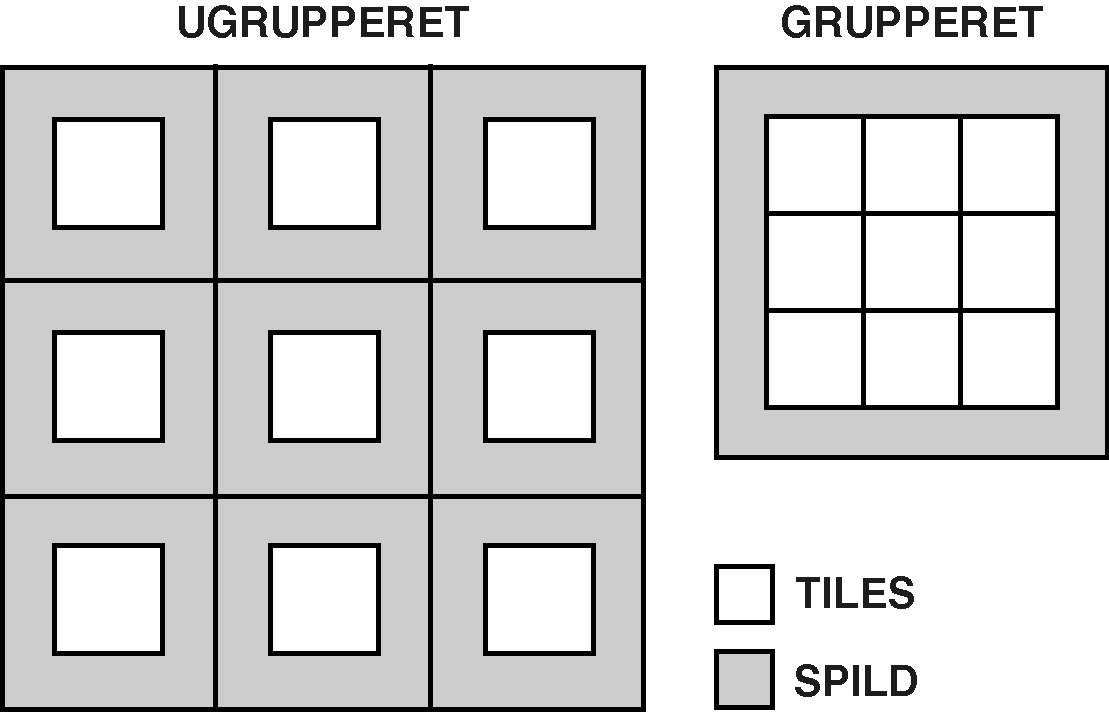
\includegraphics[width=0.5\textwidth]{visningAfKort7}
	\captionsetup{width=0.8\textwidth}
	\caption{Spild reduceres hvis tiles grupperes i rektangulære blokke.}
	\label{figur:visningAfKort7}
\end{figure}

Derudover er det væsentligt hurtigere at hente vejstykker fra quadtræerne hvis tiles grupperes til store rektangler, frem for at der hentes vejstykker for tiles enkeltvis. Grunden til dette er at vores quadtræer er optimeret således, at alle vejstykker der er i en quad og dens subquads returneres hvis den er fuldstændigt indenfor den boks der efterspørges. Det grupperede rektangel bryder med et minimalt antal quads, og er derfor langt mere effektivt, da det tager en en hel del tid at afgøre om vejstykker er inden eller uden for den efterspurgte boks.

\subsubsection{Definition af algoritme}
\label{subsec:definitionAfAlgoritme}

Vi fik hermed brug for en algoritme der kunne gruppere de tiles der endnu ikke var tegnet i rektangulære grupperinger. Algoritmen tager en liste af tiles der er er sorteret rækkevis, og efterfølgende kolonnevis, som input. Algoritmen finder det størst mulige rektangel, og tilføjer det til en liste over rektangler. Algoritmen gentager denne procedure indtil alle tiles er grupperet, og returnerer en liste af rektangler (figur~\ref{figur:visningAfKort5}).

\begin{figure}[h]
	\centering
	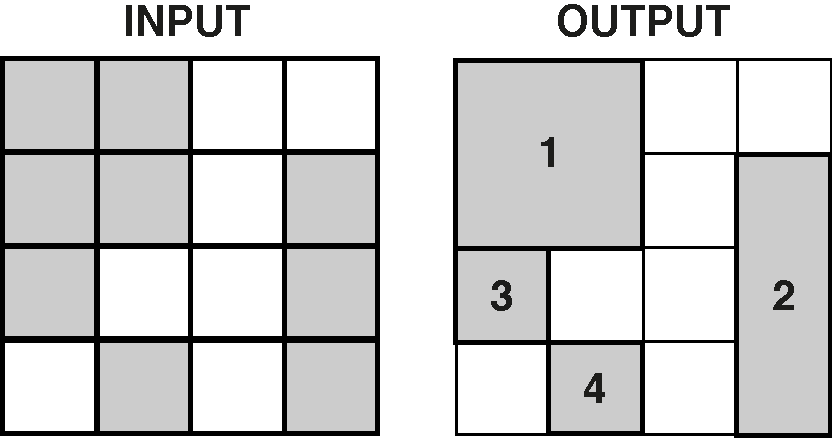
\includegraphics[width=0.5\textwidth]{visningAfKort5}
	\captionsetup{width=0.8\textwidth}
	\caption{Numrene angiver i hvilken rækkefølge rektanglerne optræder i på listen der returneres af algoritmen.}
	\label{figur:visningAfKort5}
\end{figure}

\subsubsection{Brute force: Lang tid}
\label{subsec:bruteForce}

Vores første løsningsforslag var en simpel brute force algoritme. Indledningsvist opbygger algoritmen en tabel hvor det markeres hvilke tiles der mangler at blive tegnet. Den naive løsning til dette problem er en brute-force algoritme der undersøger alle mulige rektangler i denne tabel. Hvis rektanglet er det største indtil videre og kun består af tiles der mangler at blive tegnet gemmes rektanglets position. Denne procedure gentages indtil alle mulige rektanglet er undersøgt.

\subsubsection{Dynamisk programmering: Lineær tid}
\label{subsec:dynamiskProgrammering}

Dernæst fandt vi frem tile en algoritme der løser problemet mere effektivt ved hjælp af dynamisk programmering. Ligesom brute force algoritmen opbygger den en tabel hvor det markeres hvilke tiles der mangler at blive tegnet. Herefter opbygges endnu en tabel over sammenhængende søjler ved at traversere kolonnerne i tabellen nedefra og op, og beregne højden af den enkelte søjle dynamisk (figur~\ref{figur:visningAfKort8}).

\begin{figure}[h]
	\centering
	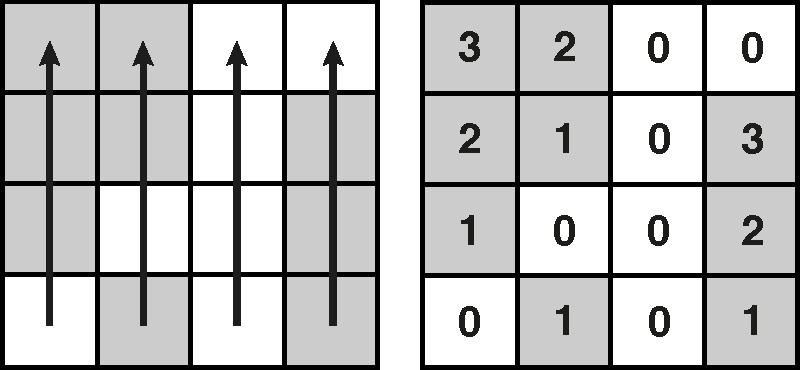
\includegraphics[width=0.5\textwidth]{visningAfKort8}
	\captionsetup{width=0.8\textwidth}
	\caption{Tabel af sammenhængende søjler opbygges.}
	\label{figur:visningAfKort8}
\end{figure}

Herefter skannes rækkerne i tabellen fra venstre mod højre, og arealet af det størst mulige rektangel der indeholder denne celle af tabellen beregnes ved hjælp af data fra søjle tabellen (figur~\ref{figur:visningAfKort9}). Undervejs i skanningen gemmes positionen af det største rektangel. Hermed en gennemgang af de første tre skridt.

\begin{itemize}
	\item \textbf{Cursoren er ved celle (1,1)}: Værdien for dette felt i søjle-tabellen er 3, og er nu højden af vores rektangel. Bredden af vores rektangel er 1, eftersom vi har undersøgt 1 felt uden at løbe ind i et felt med værdien 0 i søjle-tabellen. Arealet af det største rektangel der indeholder dette punkt er $1 * 3 = 3$, og positionen af rektanglet gemmes da det er det største indtil videre.
	\item \textbf{Cursoren er ved celle (2,1)}: Værdien for dette felt i søjle-tabellen er 2, og er nu højden af vores rektangel. Bredden af vores rektangel er 2, eftersom vi har undersøgt 1 felt uden at løbe ind i et felt med værdien 0 i søjle-tabellen. Arealet af det største rektangel der indeholder dette punkt er $2 * 2 = 4$, og positionen af rektanglet gemmes da det er det største indtil videre.
	\item \textbf{Cursoren er ved celle (3,1)}: Værdien for dette felt i søjle-tabellen er 0, og højden og bredden af vores rektangel nulstilles.
\end{itemize}

\begin{figure}[h]
	\centering
	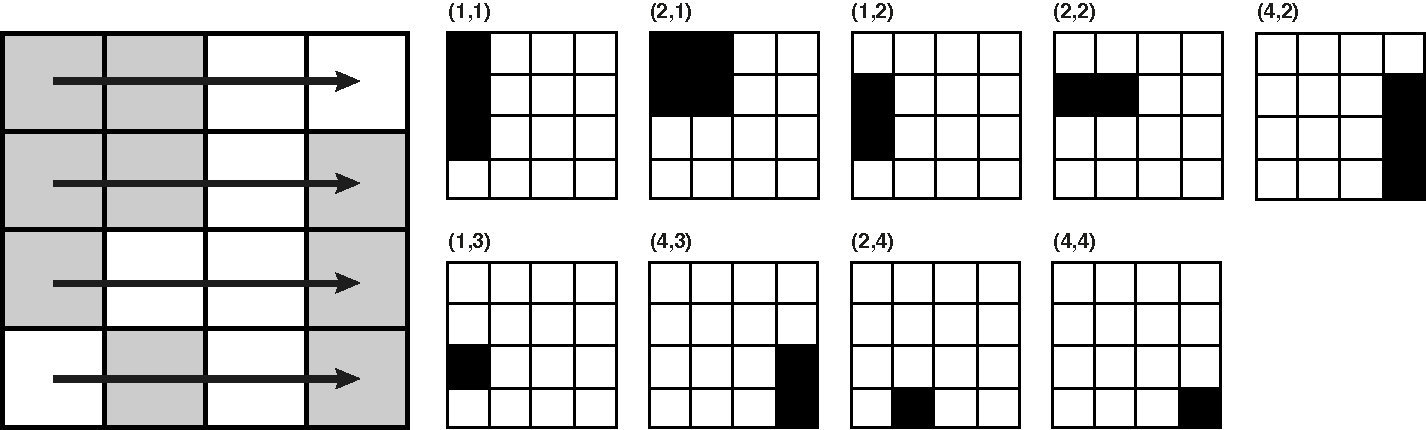
\includegraphics[width=0.9\textwidth]{visningAfKort9}
	\captionsetup{width=0.8\textwidth}
	\caption{Areal af rektangler beregnes.}
	\label{figur:visningAfKort9}
\end{figure}

Afsluttende tilføjes det største rektangel til listen af rektangler, og de tiles der udgør rektanglet markeres som tegnede.

Som følge af at vores tiles er $256 * 256$ pixels store, må det formodes at algoritmen typisk køres med N der $12*8 = 96$ eller mindre, forudsat at programmet køres i en opløsning på $(256*12) * (256*8) \approx 2880 * 1800$ pixels (MacBook Pro 15 tommer Retina skærm) eller mindre.

Den valgte algoritme kører i lineær tid $O(N)$ hvor $N$ er antallet af tiles, og blev derfor valgt til fordel for den før-nævnte brute-force algoritme som vi formoder ville have resulteret i langt længere køretider. Vi ville gerne have beregnet køretiden for brute-force algoritmen, og sammenlignet de to køretider, men dette viste sig at være meget kompliceret at beregne køretiden for brute-force algoritmen korrekt.

Et logisk argument for at den dynamiske algoritme er væsentligt hurtigere er at den efter et lineært gennemløb af cellerne kun undersøger N forskellige rektangler, hvilket skal ses i kontrast til at undersøge alle mulige rektangler. Ydermere behøver algoritmen ikke tjekke om rektanglerne udelukkende består af tiles der mangler at blive tegnet, da dette på forhånd er garanteret.

\subsubsection{Case analyse: Konstant tid}
\label{subsec:caseAnalyse}

Efter at have implementeret algoritmen der løser opgaven i alle tænkelige cases, gik vi i gang med at analysere hvilke cases der typisk opstår ofte når programmet køres i praksis, og hvilke der sjældent eller aldrig opstår (figur~\ref{figur:visningAfKort11}).

\begin{figure}[h]
	\centering
	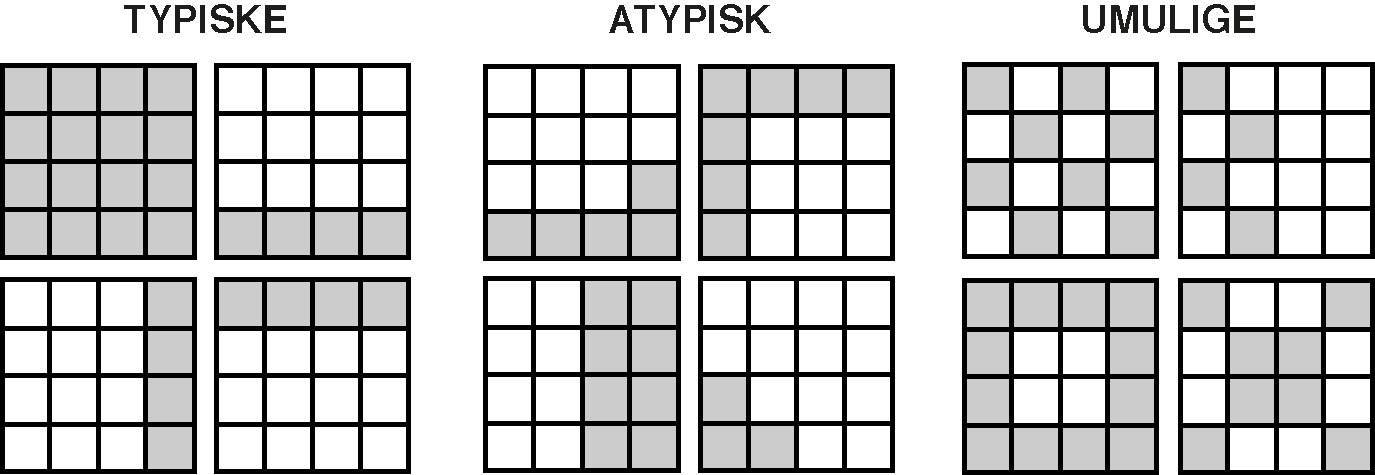
\includegraphics[width=0.9\textwidth]{visningAfKort11}
	\captionsetup{width=0.8\textwidth}
	\caption{Udvalg af typiske, atypiske og umulige cases.}
	\label{figur:visningAfKort11}
\end{figure}

Som det kan ses på figuren har vi inddelt cases i dem der er typiske og ofte sker, dem der atypiske og opstår sjældent, og dem der aldrig opstår fordi de er umulige. Korte forklaringer af udvalgte cases:

\begin{itemize}
	\item \textbf{Typisk, øverst tv.}: Brugeren har skiftet zoom-niveau, og alle tiles skal tegnes.
	\item \textbf{Typisk, øverst th.}: Brugeren har bevæget udsnittet mod nord, og en række af tiles skal tegnes.
	\item \textbf{Atypisk, øverst th.}: Brugeren har bevæget udsnittet mod nordvest, og en vinkel af tiles skal tegnes. Dette sker relativt sjældent, da det kræver at udsnittet bryder en utegnet række og kolonne samtidig.
	\item \textbf{Atypisk, nederst tv.}: Brugeren har bevæget udsnittet mod øst så hurtigt at udsnittet har brudt to utegnede kolonner samtidigt. Vi har ikke observeret dette case, men det er en mulighed.
	\item \textbf{Umulige cases}: Denne type cases er umulige fordi der er huller i dem, hvilket ikke kan lade sig gøre hvis brugeren bevæger udsnittet rundt i en kontinuerlig bane.
\end{itemize}

Følgende algoritme reducerer løser problemet i konstant tid i typiske cases, og falder tilbage på en mere tidskrævende algoritme i tilfælde af at der er tale om en atypisk case (figur~\ref{figur:visningAfKort12}):

\begin{itemize}
	\item Listen af tiles filtreres, og der oprettes en ny liste af tiles som endnu ikke er blevet tegnet.
	\item Fordi tiles er sorteret på den måde de er i den oprindelige liste, kan man lave et rektangel der går fra den første til den sidste tile fra den nye liste.
	\item Hvis antallet af tiles som rektanglet dækker over er det samme som der er utegnede tiles er problemet løst i konstant tid (figur~\ref{figur:visningAfKort12} til venstre). Hvis dette ikke er tilfældet er den pågældende case atypisk (figur~\ref{figur:visningAfKort12} til højre), og der faldes tilbage til den mere tidskrævende algoritme.
\end{itemize}

\begin{figure}[h]
	\centering
	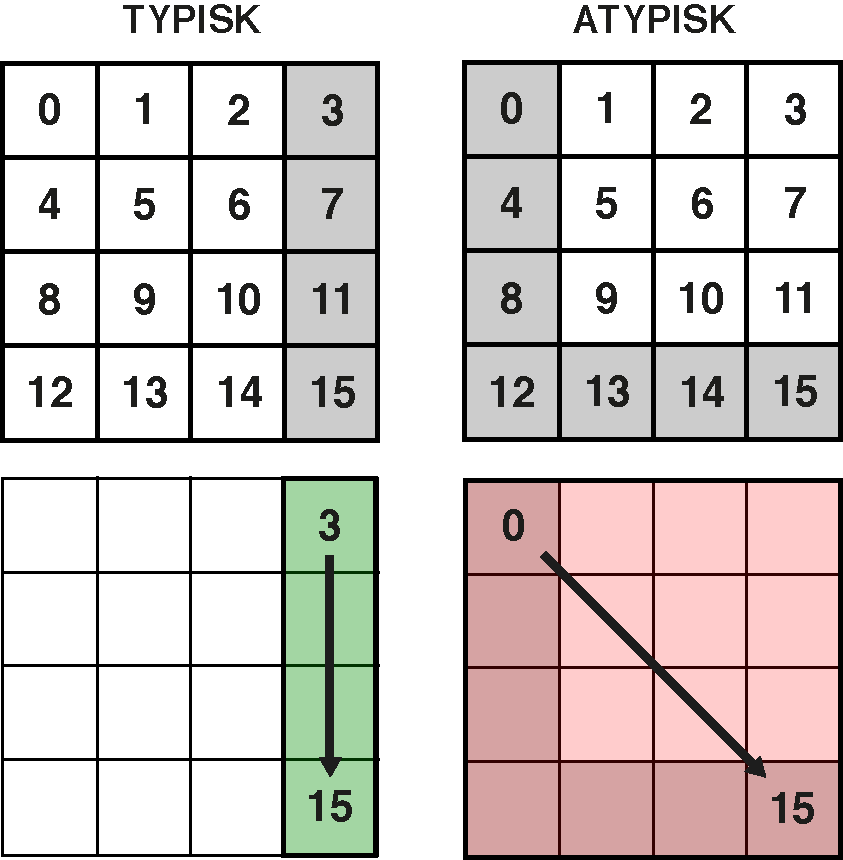
\includegraphics[width=0.5\textwidth]{visningAfKort12}
	\captionsetup{width=0.8\textwidth}
	\caption{Kørsel af algoritme på typisk og atypisk case.}
	\label{figur:visningAfKort12}
\end{figure}

Der er værd at nævne at nogle atypiske cases også løses i konstant tid af denne algoritme (f.eks. atypisk case nederst til venstre på figur~\ref{figur:visningAfKort11}). Ligeledes er det værd at nævne at algoritmen giver det forkerte svar hvis en af de ``umulige'' cases opstår, og at dette ville resultere i en fejl i programmet.

Altså endte vi i sidste ende med en algoritme der er optimeret til de specifikke forhold der gælder for vores program, og som langt det meste af tiden tager konstant tid. Det er ikke muligt at beregne en gennemsnitskøretid for algoritmen eftersom vi ikke kan forudse hvordan brugeren interagerer med kortet (hvilket afgør hvor mange atypiske cases der opstår), og det eneste der kan garanteres er derfor at køretiden i værste fald er lineær.

\subsection{Tegning af tiles}
\label{subsec:tegningAfTiles}

Når listen af rektangler er fundet, skal indholdet af hver rektangel tegnes. Følgende procedure gentages for hvert af rektanglerne (figur~\ref{figur:visningAfKort13}):

\begin{itemize}
	\item Der beregnes en boks som repræsenterer rektanglet på tiles planet.
	\item Rektanglets boks kopieres og skaleres således at den repræsenterer rektanglet på model planet.
	\item Modellen forespørges efter vejstykker der ligger indenfor boksen på model planet.
	\item Vejstykkernes koordinater skaleres til map planet, forskydes i forhold til rektanglets position, og gemmes som linjer der er klar til at blive tegnet.
	\item Linjerne tegnes til en buffer.
	\item Bufferen opdeles i tiles der gemmes i et lager.
\end{itemize}

\begin{figure}[h]
	\centering
	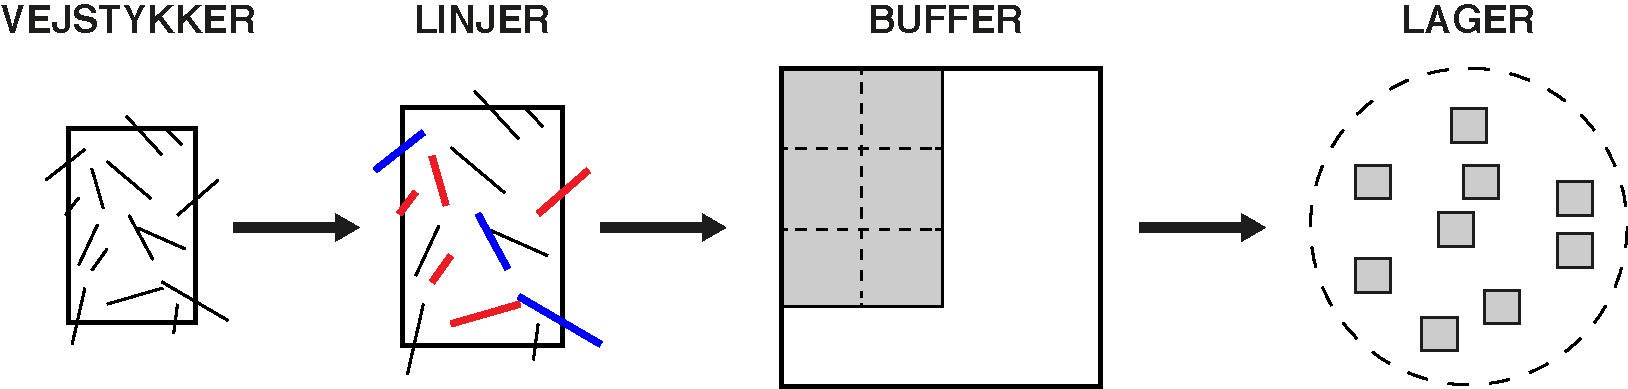
\includegraphics[width=0.9\textwidth]{visningAfKort13}
	\captionsetup{width=0.8\textwidth}
	\caption{Visualisering af proces fra vejstykker til lagring af tiles.}
	\label{figur:visningAfKort13}
\end{figure}

\subsection{Tråde}
\label{subsec:traade}

I forbindelse med tegning af tiles fandt vi det relevante at implementere tråde for at opnå følgende fordele:

\begin{itemize}
	\item Brugergrænsefladen forbliver responsiv imens nye dele af kortet tegnes på en tråd i baggrunden. Alternativet er at opgaven kører på den samme tråd som brugergrænsefladen, hvilket resulterer i at brugergrænsefladen er uresponsiv indtil tråden er færdig med at tegne.
	\item Tråde giver mulighed for at tegne flere nye dele af kortet på samme tid ved at uddelegere opgaver til forskellige tråde som køres på forskellige kerner i computerens processor.
\end{itemize}

Vi har valgt at have én tråd per kerne i forbindelse med tegning af tiles, hvilket har givet gode resultater på de maskiner vi har testet programmet på. Hver gang der skal tegnes et rektangel bliver der oprettet en ny opgave som er klar til at blive eksekveret i en tråd. Hvis der er flere opgaver end der er tråde står opgaverne i kø indtil der bliver en tråd ledig, eller eksekveres de øjeblikkeligt.

\subsection{Object pools}
\label{subsec:objectPools}

Object pools er et designparadigme der anvendes når man ønsker at genbruge objekter. Ved at bibeholde referencer til objekterne sikrer man sig at de ikke bliver smidt ud af computerens hukommelse af ``garbage collectoren''. Vi har valgt at genbruge instanser af følgende klasser i forbindelse med tegning af kortet:

\begin{itemize}
	\item \textbf{Tråde}: Tråde er dyre at initialisere, og har ikke nogen unikke egenskaber der ændrer sig under programmets levetid. Det giver derfor mening at genbruge dem så vidt muligt.
	\item \textbf{Buffers}: Bitmap buffers og de objekter der skal tegne på dem er dyre at initialisere, og det er derfor en fordel at genbruge dem.
	\item \textbf{Linjer}: Programmet har ofte brug for at have adgang til tusindvis af linjer meget hurtigt når der skal tegnes linjer til en buffer. På trods af at linje objekter er meget hurtige at initialisere, viste det sig i praksis at være en optimering at genbruge dem. Dette formoder vi skyldes at programmet har brug for store mængder af denne type objekter, og genbruger dem mange gange.
\end{itemize}

\subsection{Fake zoom}
\label{subsec:fakeZoom}

Når brugeren brugeren zoomer udsnittet ind og ud smides alle de tiles der eksisterer væk, og der er hermed nødvendigt at generere et fuldt skærmbillede af tiles for det nye zoom-niveau. Dette kan tage relativt lang tid, især hvis opløsningen af brugerens vindue er stor eller der er store mængder data indenfor udsnittet. Derfor er det i denne sammenhæng ikke praktisk at vente på at de tiles der skal vises er blevet tegnet. I stedet tegner vi et skaleret øjebliksbillede af et tidligere zoom-niveau imens der tegnes tiles i baggrunden. Ofte zoomes der mange gange på meget kort tid, og denne løsning gør det muligt hele tiden at give brugeren feedback på sit input.